\section{Program layout and functions}

The mapping of an executable to memory in Linux involves several sections:
\begin{itemize}
    \item \texttt{.plt}: this section contains stubs responsible for linking external functions.
    \item \texttt{.text}: this section contains the executable instructions of the program.
    \item \texttt{.rodata}: this section holds read-only data contributing to the program's memory image.
    \item \texttt{.data}: this section holds initialized data contributing to the program's memory image.
    \item \texttt{.bss}: this section holds uninitialized data contributing to the program's memory image. 
        The system initializes this data with zeros when the program starts running.
    \item \texttt{.debug}: this section holds symbolic debugging information.
    \item \texttt{.init}: this section holds executable instructions contributing to the process initialization code. 
        It executes before calling the main program entry point (typically named main for C programs).
    \item \texttt{.got}: this section holds the global offset table.
\end{itemize}
The program memory layout is depicted in the following simplified diagram:
\begin{figure}[H]
    \centering
    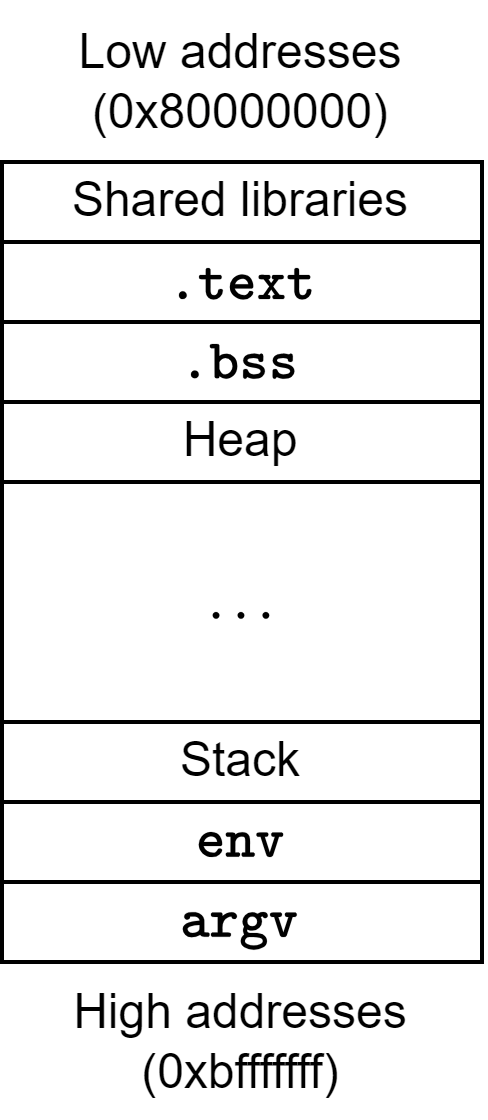
\includegraphics[width=0.18\linewidth]{images/prog.png}
    \caption{Simplified program memory layout}
\end{figure}

\subsection{Stack}
The stack operates on a Last In, First Out (LIFO) principle and is crucial for managing functions, local variables, and return addresses in programs. 
Its management is facilitated through the use of the ESP register (stack pointer). 
It's important to note that the stack grows towards lower memory addresses, which means it extends downward in the address space.

\paragraph*{Push}
To insert a new element into the stack, the following command is used:
\begin{verbatim}
push immediate or register
\end{verbatim}
This command places the immediate or register value at the top of the stack and decrements the ESP by the operand size.

\paragraph*{Push}
To remove an element from the stack, the following command is used:
\begin{verbatim}
pop destination   
\end{verbatim}
This command loads a word from the top of the stack into the destination and then increases the ESP by the operand's size.

\subsection{Functions handling}
When encountering a \texttt{call} instruction, the address of the next instruction is pushed onto the stack, and then the address of the first instruction of the called function is loaded into the EIP register.

Upon encountering a \texttt{ret} instruction, the return address previously saved by the corresponding \texttt{call} is retrieved from the top of the stack.

At the start of a function, space must be allocated on the stack for local variables. 
This region of the stack is known as the stack frame. 
The EBP register serves as a pointer to the base of the function's stack frame. 
At the function's entry point, the following steps are typically taken:
\begin{enumerate}
    \item Save the current value of EBP onto the stack.
    \item Set EBP to point to the beginning of the function's stack frame.
\end{enumerate}

Upon encountering a \texttt{leave} instruction, the caller's base pointer (EBP) is restored from the stack.

\paragraph*{Conventions}
Conventions dictate the method of passing parameters (via stack, registers, or both), the responsibility for cleaning up parameters, the manner of returning values, and the designation of caller-saved or callee-saved registers.

The high-level language, compiler, operating system, and target architecture collaboratively establish and adhere to a specific calling convention, which is an integral part of the Application Binary Interface (ABI).

In x86 C compilers, the declaration conventions are governed by the \texttt{cdecl} modifier. 
Although the \texttt{cdecl} modifier can be explicitly used to enforce these conventions, the standard rules dictate that:
\begin{itemize}
    \item Arguments are passed through the stack in a right-to-left order.
    \item Parameter cleanup is the responsibility of the caller, who removes the parameters from the stack after the called function concludes.
    \item The return value is stored in the EAX register.
    \item Caller-saved registers encompass EAX, ECX, and EDX, while other registers are considered callee-saved.
\end{itemize}
In x86 C compilers, the calling conventions follow the \texttt{fastcall} modifier. 
While explicitly using the \texttt{\_fastcall} modifier enforces these conventions, the standard guidelines dictate that:
\begin{itemize}
    \item Parameters are passed in registers: rdi, rsi, rdx, rcx, r8, and r9, with subsequent parameters passed on the stack in reverse order (caller cleanup).
    \item Callee-saved registers include rbx, rsp, rbp, r12, r13, r14, and r15.
    \item Caller-saved registers (scratch) encompass rax, rdi, rsi, rdx, rcx, r8, r9, r10, and r11.
    \item The return value is stored in rax. 
        If the return value is 128-bit, it's stored across rax and rdx registers.
\end{itemize}